%%%%%%%%%%%%%%%%%%%%%%%%%%%%%%%%%%%%%%%%%%%%%%%%%%%%%%%%%%%%%%%%%%% 
%%%%%%%%%%%%%%%%%%%%%%%%%%%%%%%%%%%%%%%%%%%%%%%%%%%%%%%%%%%%%%%%%%% 
%%%%%%%%%%%%%%%%%%%%%%%%%%%%%%%%%%%%%%%%%%%%%%%%%%%%%%%%%%%%%%%%%%% 
% \begin{frame}
%   \frametitle{Kokkos: a programming model for performance portability}

%   \only<1>{
%     \begin{itemize}
%     \item \textcolor{blue}{\textbf{Kokkos}} is a \textbf{C++ library} with \textcolor{red}{\textbf{parallel algorithmic patterns}} AND \textcolor{red}{\textbf{data containers}} for \textcolor{blue}{\textbf{node-level parallelism}}.
%     \item Implementation relies heavily on \textbf{meta-programing} to derive native {\bf low-level code (OpenMP, Pthreads, CUDA, ...)} and adapt data structure {\bf memory layout} at compile-time
%     \item Core developers at \textcolor{violet}{\bf SANDIA NL} (\textbf{H.C. Edwards, C. Trott})
%     \end{itemize}
%   }
%   \only<2>{
%     \begin{itemize}
%     \item \textcolor{darkgreen}{\textbf{Open source}}, \myurl{https://github.com/kokkos/kokkos}
%     \item Primarily developped as a base building layer for \textbf{generic high-performance parallel linear algebra} in \myhref{https://github.com/trilinos/Trilinos}{Trilinos}
%     \item Also used in molecular dynamics code, e.g. \myhref{http://lammps.sandia.gov/}{LAMMPS}
%     \item Goal: \textcolor{orange}{\textbf{ISO/C++ 2020 Standard}} subsumes Kokkos abstractions~\footnote{see mdspan proposal \myurl{https://github.com/kokkos/array_ref}}
%     \end{itemize}
%   }
%   \begin{center}
%     \includegraphics<1-2>[width=7cm]{doc/perf_portability/kokkos_summary}
%   \end{center}

% \end{frame}

%%%%%%%%%%%%%%%%%%%%%%%%%%%%%%%%%%%%%%%%%%%%%%%%%%%%%%%%%%%%%%%%%%% 
%%%%%%%%%%%%%%%%%%%%%%%%%%%%%%%%%%%%%%%%%%%%%%%%%%%%%%%%%%%%%%%%%%% 
%%%%%%%%%%%%%%%%%%%%%%%%%%%%%%%%%%%%%%%%%%%%%%%%%%%%%%%%%%%%%%%%%%% 
\begin{frame}
  \frametitle{Kokkos: a programming model for perf. portability}

  \only<1>{
    \begin{itemize}
    \item \textcolor{blue}{\textbf{Kokkos}} is a \textbf{C++ library} for \textcolor{violet}{\textbf{node-level parallelism}} (i.e. \textcolor{violet}{\bf shared memory}) providing:
 
      \begin{itemize}
      \item \textcolor{red}{\textbf{parallel algorithmic patterns}}
      \item \textcolor{red}{\textbf{data containers}} 
      \end{itemize}
    \item Implementation relies heavily on \textbf{meta-programing} to derive native low-level code (OpenMP, Pthreads, CUDA, ...) and adapt data structure memory layout at compile-time
    \item Core developers at \textcolor{violet}{\textbf{SANDIA NL}} (\textbf{H.C. Edwards~\footnote{now hired @Nvidia}, C. Trott})
    \end{itemize}
  }
  \only<2>{
    \begin{itemize}
    \item \textcolor{darkgreen}{\textbf{Open source}}, \myurl{https://github.com/kokkos/kokkos}
    \item Primarily developped as a base building layer for \textbf{generic high-performance parallel linear algebra} in \myhref{https://github.com/trilinos/Trilinos}{Trilinos}
    \item Also used in
      \begin{itemize}
      \item \myhref{http://lammps.sandia.gov/}{LAMMPS} (molecular dynamics code),
      \item \myhref{https://github.com/NaluCFD/Nalu}{NALU CFD} (low-Mach wind),
      \item \myhref{https://sparta.sandia.gov/}{SPARTA/DSMC} (rarefied gas flow),
      \item \myhref{https://github.com/SNLComputation/Albany}{Albany} (fluid/solid,...)
      \end{itemize}
      
    %\item Goal: \textcolor{orange}{\textbf{ISO/C++ 2020 Standard}} subsumes Kokkos abstractions~\footnote{\scriptsize see mdspan proposal \myurl{https://github.com/kokkos/array_ref}}
    \end{itemize}
  }
  \begin{columns}
    \begin{column}{0.34\linewidth}
      Goal: \textcolor{orange}{\textbf{ISO/C++ 2020 Standard}} subsumes Kokkos abstractions
    \end{column}
    \begin{column}{0.65\linewidth}
      \begin{center}
        \includegraphics<1-2>[width=5cm]{doc/perf_portability/kokkos_summary}
      \end{center}
    \end{column}
  \end{columns}
  \vfill
  {\scriptsize see mdspan proposal \myurl{https://github.com/kokkos/array_ref}}
\end{frame}

%%%%%%%%%%%%%%%%%%%%%%%%%%%%%%%%%%%%%%%%%%%%%%%%%%%%%%%%%%%%%%%%%%% 
%%%%%%%%%%%%%%%%%%%%%%%%%%%%%%%%%%%%%%%%%%%%%%%%%%%%%%%%%%%%%%%%%%% 
%%%%%%%%%%%%%%%%%%%%%%%%%%%%%%%%%%%%%%%%%%%%%%%%%%%%%%%%%%%%%%%%%%% 
\begin{frame}
  \frametitle{Kokkos: a programming model for performance portability}

  \begin{center}
    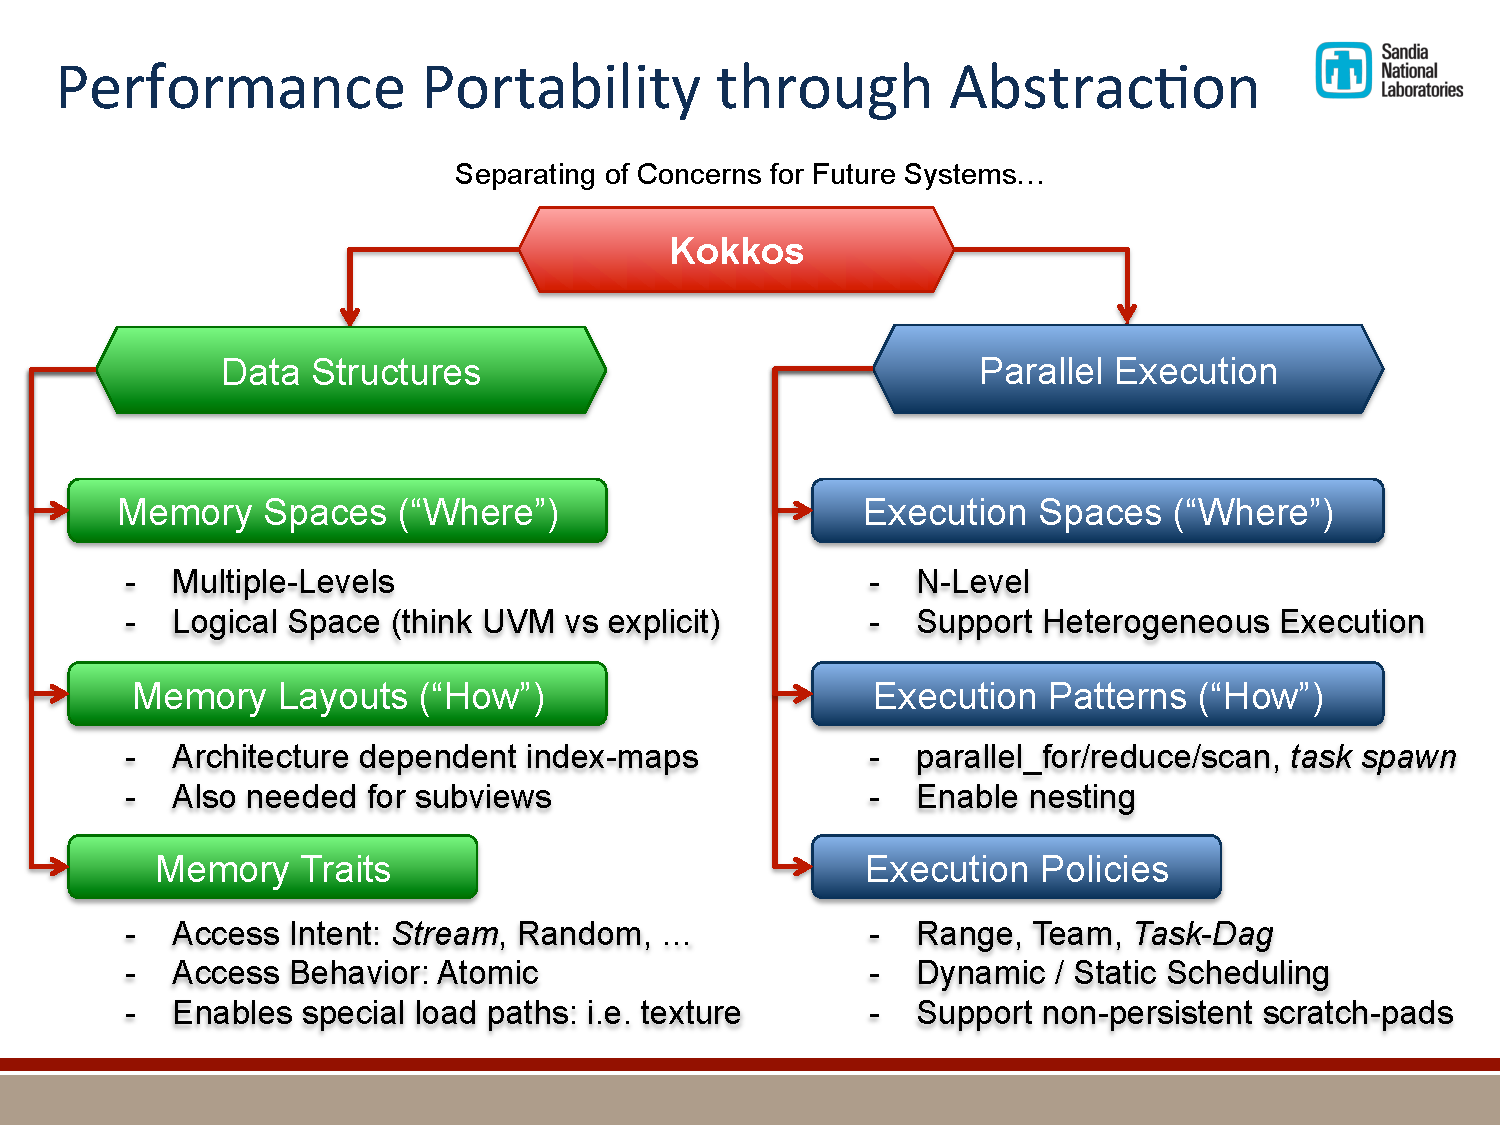
\includegraphics[width=8.0cm]{../intro/images/Kokkos-Multi-CoE_slide3}
  \end{center}

  {\small reference: \myurl{https://cfwebprod.sandia.gov/cfdocs/CompResearch/docs/Kokkos-Multi-CoE.pdf}}

\end{frame}

%%%%%%%%%%%%%%%%%%%%%%%%%%%%%%%%%%%%%%%%%%%%%%%%%%%%%%%%%%%%%%%%%%% 
%%%%%%%%%%%%%%%%%%%%%%%%%%%%%%%%%%%%%%%%%%%%%%%%%%%%%%%%%%%%%%%%%%% 
%%%%%%%%%%%%%%%%%%%%%%%%%%%%%%%%%%%%%%%%%%%%%%%%%%%%%%%%%%%%%%%%%%% 
\begin{frame}
  \frametitle{Kokkos: a programming model for performance portability}

  \begin{center}
    \includegraphics<1>[width=8.0cm]{./images/kokkos_timeline}
    \includegraphics<2>[width=8.0cm]{./images/kokkos_ecosystem}
  \end{center}

  {\small reference: \myurl{https://cfwebprod.sandia.gov/cfdocs/CompResearch/docs/Kokkos-Needs-Of-Apps.pdf}}

\end{frame}

